
%%%%%%%%%%%%%%%%%%%%%%%%%%%%%%%%%%%%%%%%%%%%%%%%%%%%%%%%%%%%%%%%%%%%%%%%%%%%%%
% Copyright (c) 2003-2015 by The University of Queensland
% http://www.uq.edu.au
%
% Primary Business: Queensland, Australia
% Licensed under the Open Software License version 3.0
% http://www.opensource.org/licenses/osl-3.0.php
%
% Development until 2012 by Earth Systems Science Computational Center (ESSCC)
% Development 2012-2013 by School of Earth Sciences
% Development from 2014 by Centre for Geoscience Computing (GeoComp)
%
%%%%%%%%%%%%%%%%%%%%%%%%%%%%%%%%%%%%%%%%%%%%%%%%%%%%%%%%%%%%%%%%%%%%%%%%%%%%%%

\section{Point Sources}
\label{POINT SOURCES}
In the chapter we will show the usage of point sources and sinks. 
A simple example is a blockm of material with heat source at a location
$p$ and heat sink at a location $q$. Under the assumption of a constant
conductivity the steady heat diffusion equation for the temperature $u$
is given as 
\begin{equation}
        -u_{,ii} = s(p_{in}) \; \delta_{p_{in}} + s(p_1) \; \delta_{p_1}
        \label{EX:DIRAC1}
\end{equation}
where $\delta_{p_{in}}$ and $\delta_{p_{out}}$ refer to the Dirac $\delta$-function and
$s({p_{in}})$ and $s({p_{out}})$ define the heat production and heat extraction rates at 
locations ${p_{in}}$ and ${p_{out}}$, respectively.

First the locations of  point sources and sinks need to be added to the 
domain. This is done at generation time:  
\begin{python}
mydomain=Rectangle(30,30, l0=3, l1=2, 
                diracPoints=[(1.,1.), (2.,1.)],  diracTags=['in', 'out'])
\end{python}
In this case the points are located at $p_{in}=(1.,1.)$ and $p_{out}=(2.,1.)$.
For easier reference the points are tagged with the name \var{in} and \var{out}. 

The values at the point source locations are defined using a \Data object. One possible
way to define the values at the locations defined through the \var{diracPoint} list is using tagging: 
\begin{python}
s=Scalar(0., DiracDeltaFunctions(mydomain))
s.setTaggedValue('in', +1.)
s.setTaggedValue('out', -1.)
\end{python}
Here we set value $1$ at locations tagged with \var{in} (in this case this is just point $p_{in}=(1.,1.)$ ) and value $-1$ at locations tagged with \var{out} (in this case this is just point $p_{out}=(2.,1.)$). The point source in the right hande side of the PDE~\eqn{EX:DIRAC1} is then set as
\begin{python}
mypde = LinearSinglePDE(domain=mydomain)
mypde.setValue(y_dirac=s)
\end{python}
Under the assumption that we fix the temperature to zero on the entire boundary 
the script to solve the PDE is given as follows:
\begin{python}
from esys.escript import *
from esys.weipa import *
from esys.finley import Rectangle
from esys.escript.linearPDEs import LinearSinglePDE

mydomain=Rectangle(30,30, l0=3, l1=2, 
                diracPoints=[(1.,1.), (2.,1.)],  diracTags=['in', 'out'])
x = mydomain.getX()
gammaD = whereZero(x[0])+whereZero(x[1])+whereZero(x[0]-3.)+whereZero(x[1]-2.)

s=Scalar(0., DiracDeltaFunctions(mydomain))
s.setTaggedValue('in', +1.)
s.setTaggedValue('out', -1.)

mypde = LinearSinglePDE(domain=mydomain)
mypde.setValue(q=gammaD, A=kronecker(2), y_dirac=s)
u = mypde.getSolution()
saveVTK("u.vtu",sol=u)
\end{python}
%
Result is shown in Figure~\ref{FIG:EX:DIRAC}.
%
\begin{figure}[ht]
\center
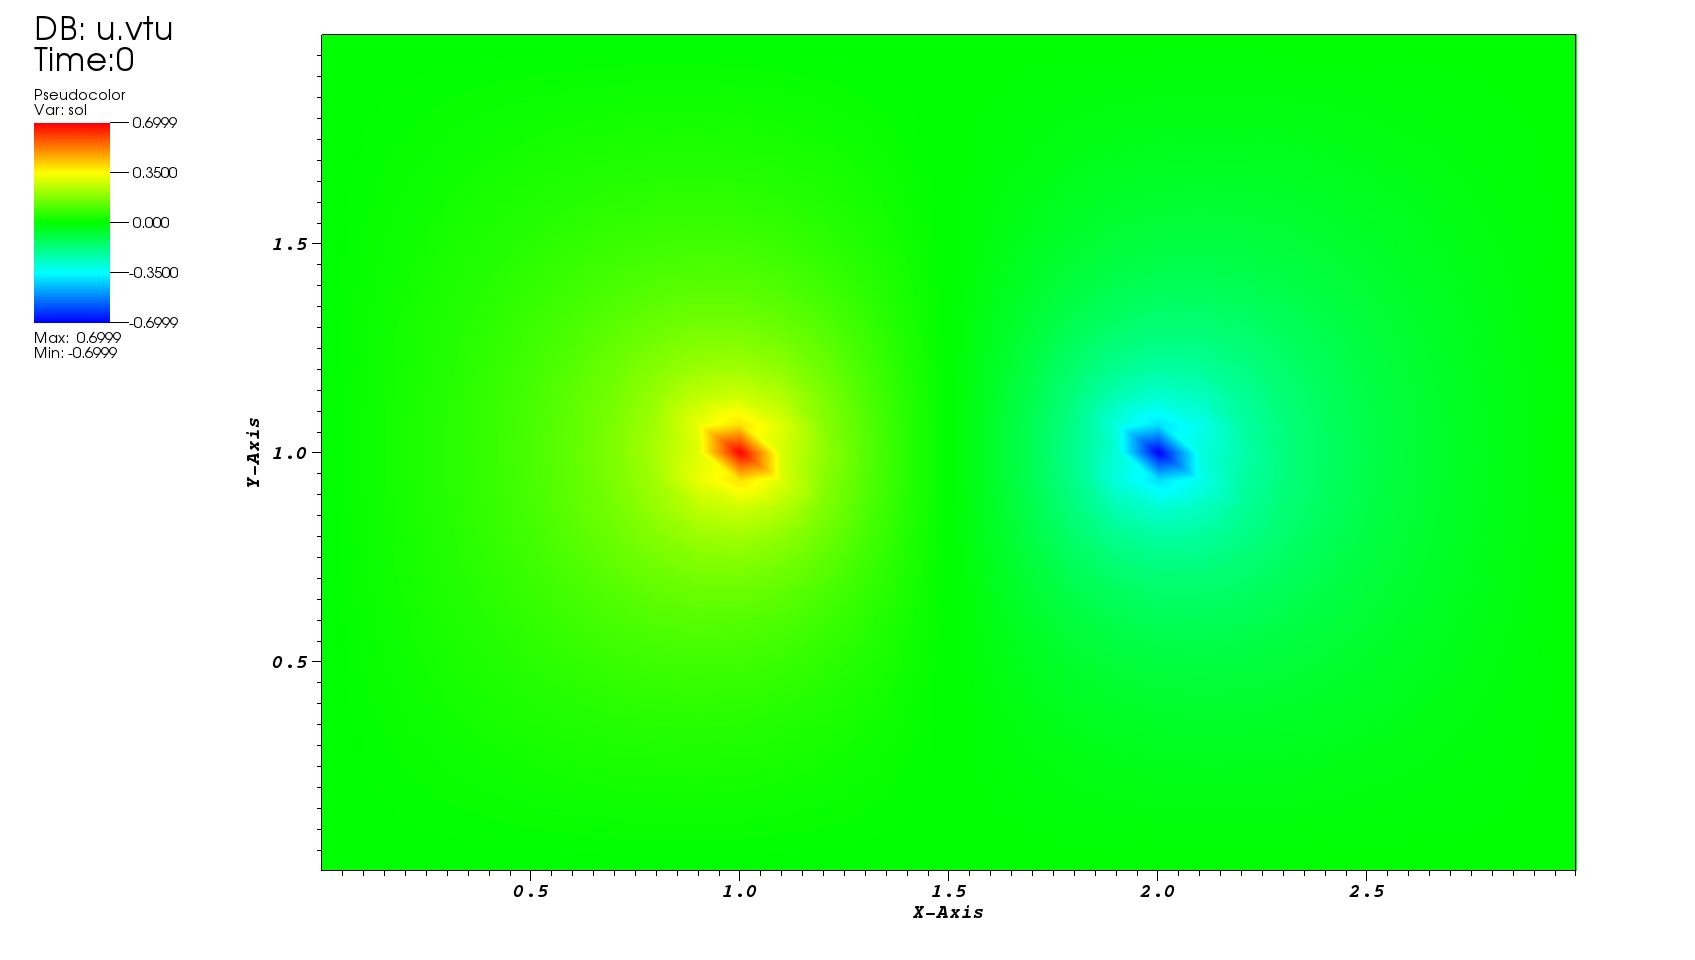
\includegraphics[height=5cm]{diracplot}
%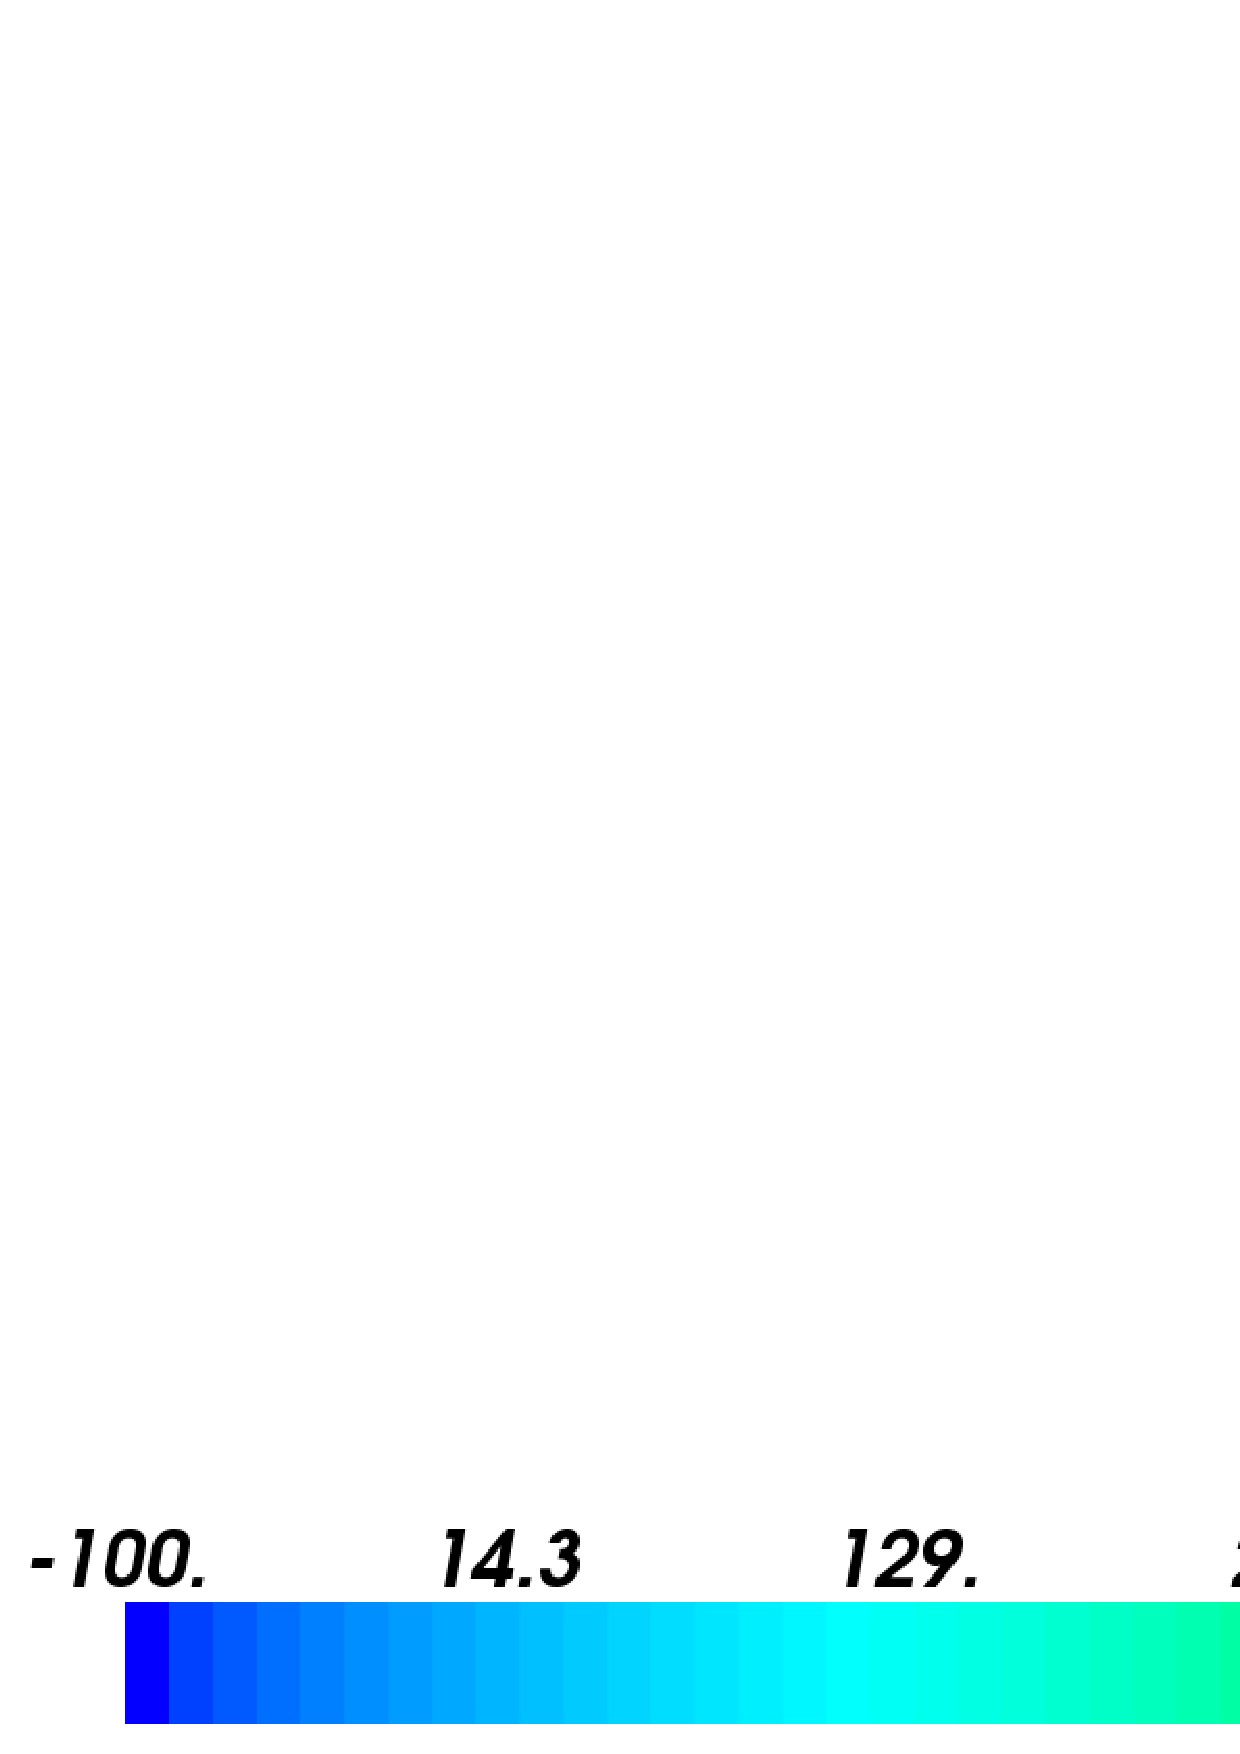
\includegraphics[scale=0.25]{stokes-fluid-colorbar}
\caption{Results diffusion problem with nodal source and sink.}
\label{FIG:EX:DIRAC}
\end{figure}

